\documentclass[conference]{IEEEtran}
\IEEEoverridecommandlockouts

% Packages
\usepackage{cite}
\usepackage{subcaption}
\usepackage{amsmath,amsfonts}
\usepackage{algorithm}
\usepackage{algpseudocode}
\usepackage{graphicx}
\usepackage{textcomp}
\usepackage{xcolor}
\usepackage{booktabs}
\usepackage{adjustbox}
\usepackage{listings}
\usepackage{hyperref}
\usepackage{verbatim}
\usepackage{multirow}
\usepackage{placeins}

\newcommand{\todo}[1]{\color{red} TODO #1\color{black}}
\newcommand{\torem}[1]{\color{olive} #1 \color{black}}

\def\BibTeX{{\rm B\kern-.05em{\sc i\kern-.025em b}\kern-.08em
    T\kern-.1667em\lower.7ex\hbox{E}\kern-.125emX}}



\begin{document}

\title{Second Deliverable report \\
\footnotesize \textit{"Matteo Di Noia": Mat: 258426, \texttt{matteo.dinoia@unitn.it}, GitRepo: \texttt{\href{https://github.com/matteo-dinoia/GPU-Computing-2025-258426}{matteo.dinoia/GPU-Computing-2025-258426}}}}

\maketitle

\begin{abstract}
%\torem{[max 200 words]}\\
The sparse matrix-dense vector multiplication (SpMV) is a common linear algebra operation consisting of a matrix multiplication between, as the name implies, a sparse matrix and a dense vector. SpMV is widely used in many real-world applications such as scientific computing and graph analytics.

This paper covers one of the possible representation used for sparse matrix in SpMV, COO. Of this problem, this paper quickly discuss CPU implementation and then focuses on GPU implementation, both naive version and more advanced versions using prefix sum, shared memory and warp operation. To do so we will need to add some sorting assumption to COO. Finally, the various results are compared and are suggested combination of the best kernels with some heuristic.
\end{abstract}

\begin{IEEEkeywords}
Sparse Matrix, SpMV, CUDA, Parallelization, Storage Format, Prefix Sum
\end{IEEEkeywords}

\section{Introduction}
%\torem{[max 300 words]Introduce SpMV application and its parallelization challenges \dots}\\

Sparse matrix vector multiplication (SpMV) is a core computation that is at the foundation of every implicit sparse linear algebra solver. It is also one of the most common primitive in scientific computing, and graph analytics, eg. it is present in software such as MatLab and Numpy.

Due to being an intrinsically memory-bound algorithm, its performance are limited by the bandwidth between the process and the memory, especially on highly parallelized, throughput-oriented architectures such as GPU.


\section{Problem Statement}
%\torem{Define the problem statement, including a description of the storage format used and a brief discussion of the parallelization approach (e.g., using CUDA).}
Sparse matrix vector multiplication (SpMV) is a matrix multiplication between a matrix $A$ of size $n\times m$ and a vector $x$ of size $m\times 1$, which result in a vector $y$ of size $n\times 1$ computed as follows:

\[y=A \cdot x\]
\[y_i = \sum_{k=1}^{n}A_{ik} x_{k}\]

\begin{figure}[h!]
	\centering
	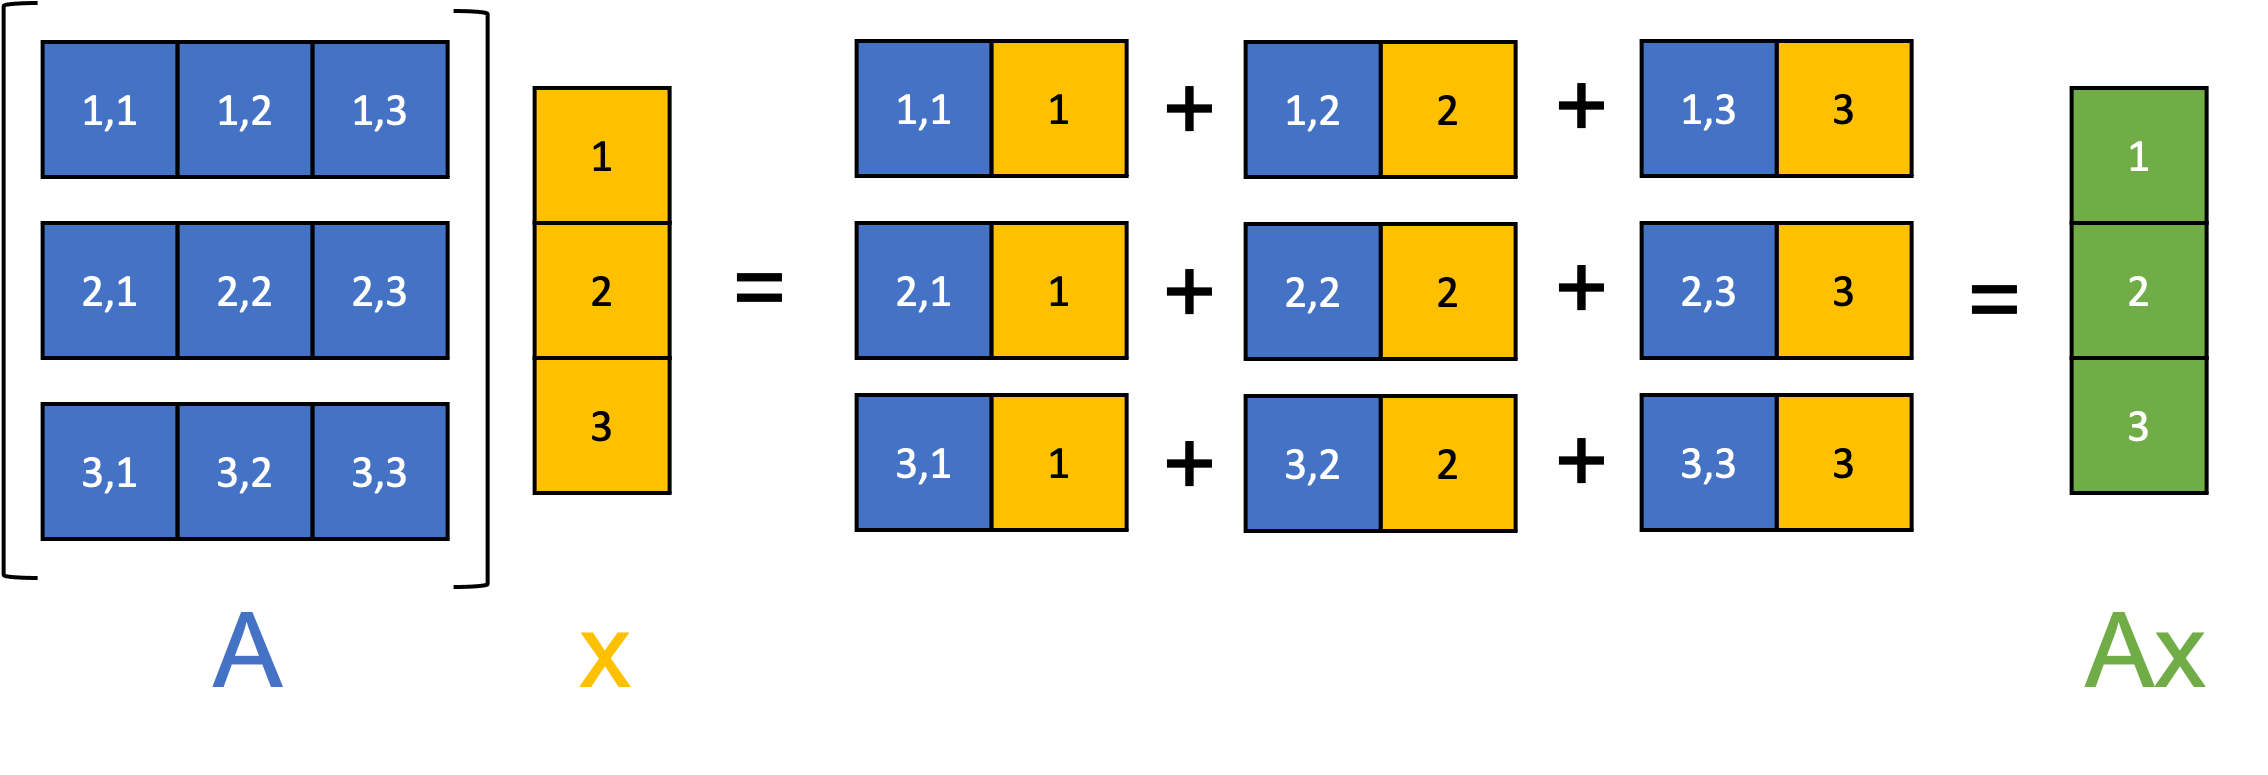
\includegraphics[width=0.9\linewidth]{other_img/matrix_vec_mult}
	\caption{Matrix Vector Multiplication}
	\label{fig:matrixvecmult}
\end{figure}
%TODO reference https://mbernste.github.io/posts/matrix_vector_mult/

The particularity of Spmv, is that the matrix is sparse, meaning that most of its elements are empty (contains zero) and while the vector is dense, as in not sparse.



An efficient implementation of SpMV present various challenges, most of which are related to choosing a good storage format and having an efficient memory access. The latter of which, is required because, as mentioned before, SpMV is a memory-bound algorithm. In fact the arithmetic intensity, meaning the worst-case ratio between the number of arithmetic operation over the number of read/write operation , is very low:
\[Intensity = \frac{2\ flop}{6 \cdot 4\ bytes} = 0.083\frac {flop}{bytes}\]
Instead the role of the storage format, during the program execution, is to facilitate such access.

\subsection{Storage Format}
%\torem{Details about the format (e.g., CSR, COO, etc.) \dots}

Multiple format exists such as Compressed Sparse Row (CSR), Coordinate (COO), ELLPACK (ELL), etc. In the present paper, the analysis is concentrated over the COO format. The latter is the simplest one, in which three array are used to represent the matrix:

\begin{figure}[h!]
	\centering
	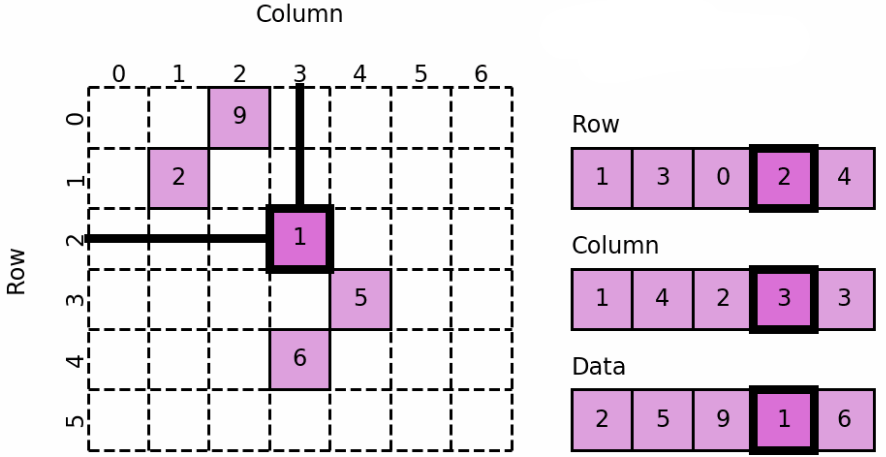
\includegraphics[width=0.9\linewidth]{other_img/coo}
	\caption{Example of COO format}
	\label{fig:coo}
\end{figure}
% TODO reference https://firas-jolha.github.io/bigdata2025/html/bs/BS%20-%20Lab%208%20-%20Apache%20Spark%20MLlib.html

\begin{itemize}
	\item \textbf{rows (/Ys)}: containing for every $i$ the row (or $y$ value), in which the $i$-th element of the matrix is;
	\item \textbf{cols (/Xs)}: containing for every $i$ the column (or $x$ value), in which the $i$-th element of the matrix is
	\item \textbf{values (/data)}: containing for every $i$ the value of $i$-th element;
\end{itemize}

While the COO format may have no sorting guarantees, during the analysis of this paper it will be assumed the use of a COO sorted by row index and then by column index. This is required as the optimized kernel using prefix-sum are based on that assumption.
\[el1 < el2 := row1 < row2 \lor (row1 = row2 \land col1 < col2) \]

This make the format, partially, similar to Compressed Row Format (CSR); with the difference that in CSR the row vector is compressed, as the name implies, to an array contains pointers that mark the beginning of rows within the column and value array. CSR format will also be mentioned as point of comparison of the CPU implementation.

\todo{Add image of sorted COO and CSR}

\subsection{Parallelization}
%Describe the CUDA implementation approach \dots
Being SpMV a conceptually easy operation, in order to parallelize it we can exploit independence between operation on some blocks of data, to obtain data parallelism.

The simplest way to split the data and to parallelize the operation, is to have a thread for each element in the COO format. This is simple but while the read operation on the matrix and the multiplying vector are not interfering; the write, in particular it is a read followed by an addition and finally a write, to the result vector can happen at the same time another thread is doing the same time it is accessing the same location. This is a race condition and to avoid it, atomic operations are required. The operation in question needed is $atomicAdd$, which perform read, addition and write atomically.

\begin{figure}[h!]
	\centering
	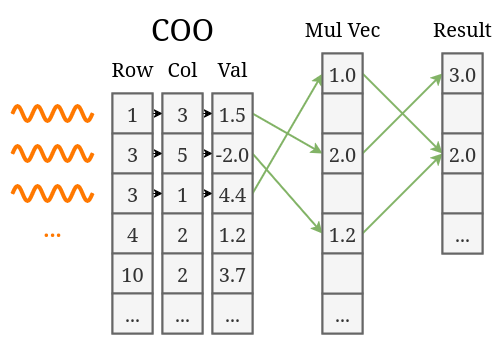
\includegraphics[width=0.7\linewidth]{other_img/diagram-threads}
	\caption{Simple parallelization idea and its faults}
	\label{fig:diagram-threads}
\end{figure}


But this approach has some limitations: the small but existing overhead of the atomic operation; but mostly the great amount of writing to same cell in the result vector. We can tackle the second one by exploiting the fact that to compute the product of a row and the vector it is only needed read access to the previous two and write access to a single element of the result vector.
\begin{figure}[h!]
	\centering
	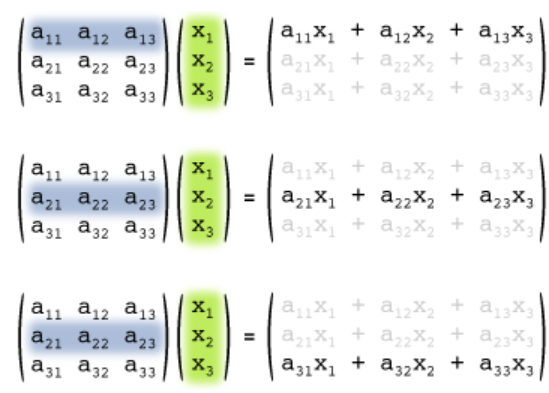
\includegraphics[width=0.7\linewidth]{other_img/row-independence}
	\caption{Eg. rows independence of matrix vector multiplication  }
	\label{fig:row-independence}
\end{figure}

Because of this we can have a single write for each row, possibly decreasing the amount of write if there are more than a single entry for row. But the major improvement of this method is that we reduce the number of time we write on the same location, which improve performance, especially when using $AtomicAdd$, because when multiple write are performed only one can succeed while the other need to wait.

\section{State of the Art}
The state of art SpMV for CPU is OpenBLAS, which is an optimized BLAS (Basic Linear Algebra Subprograms). On the other hand, cuSPARSE is a Cuda based GPU accelerated BLAS which perform significantly faster than CPU only alternatives thanks to the higher degree of parallelization.
\todo{add more}

\section{Methodology and Contributions}\label{sec:methodology}

%describe the methodology used during the analysis, the compared algorithms and the expected outcomes. Use pseudo-codes like Algorithm \ref{alg:COOaggr} to describe your own implemented kernels.

%\noindent Include at least the following implementations:
%\begin{itemize}
%    \item Naive CPU implementation
%    \item Optimised CPU implementation based on cache behaviour
%    \item GPU naive implementation
%\end{itemize}

For the analysis, a COO CPU \ref{alg:COO_CPU} and  naive GPU \ref{alg:COO_GPU} implementations were created. Both access data in the sparse matrix $A$ sequentially and the resulting vector $Y$ sequentially, sacrificing instead the sequentiality in the access of the dense multiplying vector $v$.

\begin{algorithm}[h!]
	\caption{COO SpMV on CPU}
	\algorithmicrequire~The input vectors $Ar$, $Ay$, $Av$ representing the COO matrix of size $nnz$, the vector $X$ of size $nrows$.
	\begin{algorithmic}[1]
		\Procedure{Function}{$Ar$, $Ay$, $Av$, $X$, $nnz$}
		\For{$k$ in $\{1 \dots nnz\}$}
		\State $Y[Ay[k]] = Y[Ay[k]] + Av[k] * X[Ax[k]] $\label{partitioning}
		\EndFor
		\State \textbf{return} $Y$\Comment{the result vector}
		\EndProcedure
	\end{algorithmic}
	\label{alg:COO_CPU}
\end{algorithm}

We also implemented a CSR CPU implementation to have a point of comparison for the CPU version. Because of the size difference between CSR and COO, with CSR being smaller because of the compressed rows array, we expect the throughput of the latter to be greater than the one of COO as both are memory-bound application.

\begin{algorithm}[h!]
	\caption{CSR SpMV on CPU}
	\algorithmicrequire~The input vectors $Ar$, $Acy$, $Av$ representing the CSR matrix of size $nnz$, the vector $X$ of size $nrows$.
	\begin{algorithmic}[1]
		\State $k \leftarrow 0$
		\Procedure{Function}{$Ar$, $Acy$, $Av$, $X$, $nnz$, $nrows$}
		\For{$r$ in $\{1 \dots nrows\}$}
		\State $end \leftarrow Acy[r + 1]$
		\While{$k < end$}
		\State $Y[r] \leftarrow Y[r] + Av[k] * X[Ax[k]] $\label{partitioning}
		\State $k \leftarrow k + 1$
		\EndWhile
		\EndFor
		\State \textbf{return} $Y$\Comment{the result vector}
		\EndProcedure
	\end{algorithmic}
	\label{alg:CSR_CPU}
\end{algorithm}

The simple CPU version \ref{alg:COO_CPU} can be parallelized, in order to make a baseline GPU version. This can be done by simply parallelizing the for, having a thread for each element of the matrix and replacing the assignment and addition with a $atomicAdd$, as shown in the following pseudo-code \ref{alg:COO_GPU} .

\begin{algorithm}[h!]
	\caption{GPU baseline COO SpMV}
	\algorithmicrequire~The input vectors $Ar$, $Ay$, $Av$ representing the COO matrix of size $nnz$, the vector $X$ of size $nrows$.
	\begin{algorithmic}[1]
		\Procedure{Function}{$Ar$, $Ay$, $Av$, $X$, $nnz$}
		\For{$k$ in $\{1 \dots nnz\}\ \textbf{parallel}$}
		\State $atomicAdd(Y[Ay[k]],\ Av[k] * X[Ax[k]]) $\label{partitioning}
		\EndFor
		\State \textbf{return} $Y$\Comment{the result vector}
		\EndProcedure
	\end{algorithmic}
	\label{alg:COO_GPU}
\end{algorithm}

\todo{CHANGE But this simplicity comes with a cost: performance. In fact, atomic operation are never cheap and as such it is expected that this algorithm will not even be close to the theoretical worst-case, instead it will be much worse.

But, there are some possible change that can be done to reduce cache missed and improved performance, as detailed in the following chapters.}

\todo {add more pseudo code and co}

\section{System Description and Experimental Set-up}
%Use this section to describe system, dataset and experimental set-up.

\subsection{System Description}
%Describe the used system and the software environment (CUDA version, GCC version, \dots). Decide which information are valuable to group into a table like Table \ref{tab:system_description} and which are more valuable to be described in the text.

The previous algorithms were tested with GCC 12.3, CUDA version 12.5 on the $Baldo$ cluster in the partition $edu$-$short$ only on the node $edu01$. That means the program were run on a system with a "AMD EPYC 9334" 32-Core CPU and as a GPU a "NVIDIA A30", the attributes of the latter can be seen in Table \ref{tab:system_description}.

\begin{table}[h!]
	\centering
	\begin{adjustbox}{width=0.8\columnwidth}
		\begin{tabular}{lc}
			\toprule
			\textbf{Metrics} &  \textbf{Value}  \\
			\midrule
			Memory Size & 24 GB \\
			Peak FP32 Compute &  10 TFlops   \\
			Peak Memory Bandwidth (HBM2) & 933 GBs  \\
			Maximum number of threads per block & 1024 \\
			Maximum \# of block per grid & 2147483647 \\
			Warp size & 32 \\
			SM counts & 56\\
			\bottomrule
		\end{tabular}
	\end{adjustbox}
	\vspace{1em}

	\caption{System details}
	\label{tab:system_description}
\end{table}

From this information, it is possible to gather that neither memory size nor peak FP32 operation will be a bottleneck as the matrix are at most some gigabyte once loaded in memory and the algorithm is low algebraic intensity. We can also note that the the number of block is limited to 1024, while the number of blocks is so large that for our use can be considered infinite, which we will do when using the baseline kernel. Finally, we notice the count of SM (Simultaneous Multiprocessor) which we will need to saturate to reach full performance, and the maximum memory bandwidth which will be the theoretical limiting factor of performance.



\subsection{Dataset description}

%Describe the used dataset and the reasons of your choice. List the used input matrices and all the information that you think are valuable to show (number of non-zero elements, sparsity ratio, \dots); Table \ref{tab:dataset} gives you a possible example.
To test the implementations we use six datasets \ref{tab:dataset} .
\begin{table}[h!]
	\centering
	\begin{adjustbox}{width=0.9\columnwidth}
		\begin{tabular}{lrrrr}
			\toprule
			\textbf{Dataset} & \textbf{Density} & \textbf{Non-zero} & \textbf{Per row} & \textbf{Per row} \\
			&  \textbf{ } &  & \textbf{ (avg)} & \textbf{ (max)} \\
			\midrule
			mawi\_201512020330 & $10^{-6}\%$ & 480M & 2.1 & 210M \\
			circuit5M\_dc & $10^{-4}\%$ & 14M & 5.4 & 27 \\
			delaunay\_n23 & $10^{-4}\%$ & 50M & 6.0 & 28\\
			model7  & $0.16\%$ & 51k & 15.2 & 253\\
			hugetrace-00000 & $10^{-5}\%$ & 6.9M & 1.75 & 3\\
			europe osm & $10^{-6}\%$ & 108M & 2.1 & 13\\
			mouse\_gene & $1.4\%$ & 29M & 642 & 8k\\
			mycielskian16 & $1.3\%$ & 33M & 679 & 25k \\
			\bottomrule
		\end{tabular}
	\end{adjustbox}
	\vspace{1em}

	\caption{Datasets used in the analysis}
	\label{tab:dataset}
\end{table}

 The largest one \textit{Mawi}, is also the one with some row and cols that are very dense, because of this we expect it to be \todo{continue here and after}. Of medium size there are Delaunay with radial elements and Circuit5M which is a mixture of the previous two. Finally the smallest is Model7 with somewhat irregular patterns.
\FloatBarrier
\begin{figure}[h!]
	\centering
	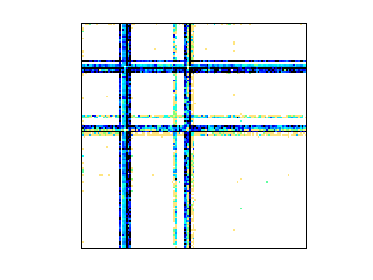
\includegraphics[width=0.3\linewidth]{model_images/mawi_201512020330}
	\label{dat:mawi}
	~
	\includegraphics[width=0.3\linewidth]{model\_images/circuit5M\_dc}
	\label{dat:circuit}

	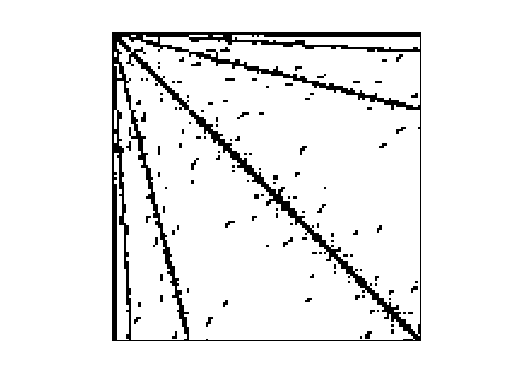
\includegraphics[width=0.3\linewidth]{model_images/delaunay_n23}
	\label{dat:delaunay}
	~
	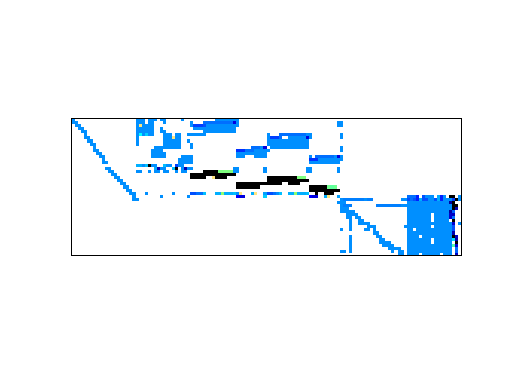
\includegraphics[width=0.3\linewidth]{model_images/model7}
	\label{dat:model7}

	\caption{In the top, the visualization of Mawi and Circuit5c and in the bottom Delaunay and Model7}
	\label{img:data-vis}
\end{figure}





\FloatBarrier

\section{Experimental Results}
%Present and discuss results. Include plots and tables when required (like Figure \ref{fig:enter-label}). Do not simply describe the figures; criticise the achieved results by underlining how they confirm/differ from the expected outcomes described in Section \ref{sec:methodology}.

%\noindent For the analysis include
%\begin{itemize}
%	\item Valgrind and runtime comparison between the CPU implementations
%	\item Runtime CPU vs GPU comparison looping over different matrix dimensions
%\end{itemize}
\subsection{CPU implementations}
We measured the average time (over 20 cycles with 5 warmup), and as the figure \ref{fig:time-cpu-results} shows, CSR is faster than the COO implementation in most cases. In particular, over the datasets we measured the CSR implementation is 2.48 times faster (+148\%) on average.

\begin{figure}[h!]
	\centering
	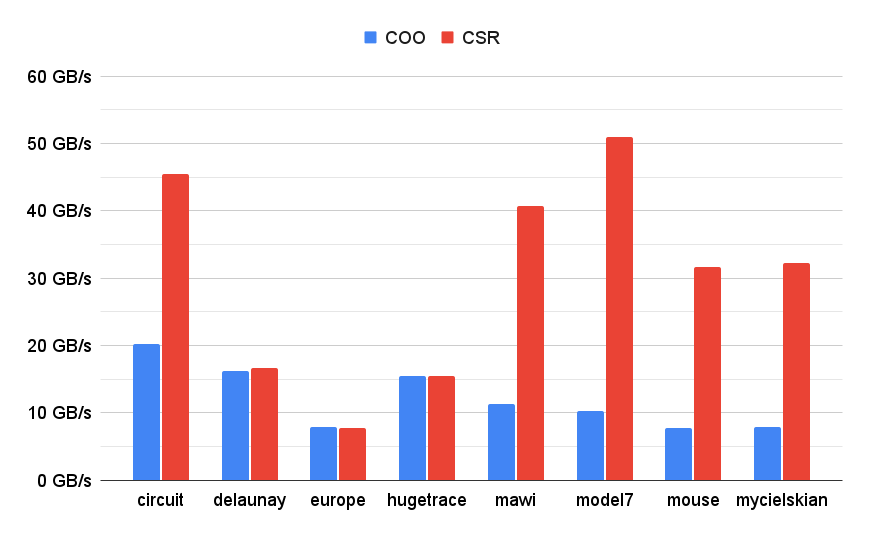
\includegraphics[width=1\linewidth]{data_images/cpu}
	\caption{CPU implementations performance over datasets}
	\label{fig:time-cpu-results}
\end{figure}

In the Table \ref{tab:time-cpu-results} are also reported the bandwidth calculated from the average times, instead of the flops, that is because it is memory bound, so we care more about bandwidth. As it possible to see, CSR win in almost every case (by up to 5x in Model7), except for Hugetrace where it ties with COO and in Europe where COO is 0.38\% faster which is in the range of error.

\begin{table}[h!]
	\centering
	\begin{adjustbox}{width=0.9\columnwidth}
		\begin{tabular}{lcccc}
			\toprule
			\textbf{Datasets} & \textbf{COO} & \textbf{COO} & \textbf{CSR} & \textbf{CSR} \\
			& \textbf{(ms)} & \textbf{(GBs)} & \textbf{(ms)} & \textbf{(GBs)} \\
			\midrule
			circuit & 22.71 & 20.28 & 10.12655 & 45.49 \\
			delaunay & 74.83 & 16.14 & 72.76855 & 16.60 \\
			europe & 331.19 & 7.83 & 332.649 & 7.80 \\
			hugetrace & 10.63 & 15.54 & 10.62155 & 15.54 \\
			mawi & 1015.80 & 11.34 & 282.75595 & 40.75 \\
			model7 & 0.12 & 10.27 & 0.02405 & 50.92 \\
			mouse & 88.93 & 7.82 & 21.93315 & 31.70 \\
			mycielskian & 102.37 & 32.16 & 24.88275 & 32.20 \\
		\end{tabular}
	\end{adjustbox}
	\vspace{1em}

	\caption{CPU implementations performance over datasets}
	\label{tab:time-cpu-results}
\end{table}


Using Model7 as datasets to test cache misses, the results are the one in the Table \ref{tab:cache-results} . These values are very rough as cachegrind doesn't allow testing of a single portion of code. As such, both test were conducted in the same exact codebase with the single difference of calling COO or CSR methods (so even the conversion from COO to CSR was done in both).

This minimize the difference between the test but doesn't solve the issue of the initialization causing some misses. To reduce the impact of the initial misses, the SpMV was compute 500 times.

As expected, CSR having the rows array compressed, cause less lower reference to memory location and so it also cause slightly less cache misses.
\begin{table}[h!]
	\centering
	\begin{adjustbox}{width=\columnwidth}
		\begin{tabular}{lrrrrc}
			\toprule
			\textbf{Type} & \textbf{D Refs} & \textbf{D1 misses} & \textbf{LLd misses} & \textbf{D1 miss rate} & \textbf{LLd miss rate} \\
			\midrule
			COO & 429M & 5.35M & 13.4k & 1.2\% & 0.0\% \\
			CSR & 38M & 4.03M & 13.4k & 1.1\% & 0.0\% \\
			\bottomrule
		\end{tabular}
	\end{adjustbox}
	\vspace{1em}

	\caption{Valgrind's cachegrind tool results}
	\label{tab:cache-results}
\end{table}

Those are likely the major reason causing the COO, implementations to be slower, as all the rest is the same. In fact, as said before, here the COO is assumed to be sorted and as such the executions differ only by the memory access to the row of the two formats.

\subsection{GPU implementations}
The simple idea of a GPU Algorithm \ref{alg:COO_GPU} can be implemented in various ways. The versions tested in this paper are:
\begin{itemize}
	\item \textbf{"Kernel 1 size"}: where each thread acquires locally adjacent elements;
	\item \textbf{"Kernel threads size"}: where the distance between an element and the next that the thread acquire is the \# threads;
	\item \textbf{"Kernel warp size"}: where the distance between an element and the next that the thread acquire is the size of a warp;
	\item \textbf{"Kernel block size"}: where the distance between an element and the next that the thread acquire is the size of a block;
\end{itemize}

It was, then, tested the performance of them, with respect to the number of thread per block and the number of blocks. As expected the first kernel is the worst one and warp size and block size are in the first place, while perform around the same. This is because of the fact that warp share cache and as such threads in same thread should access close position. The reason for "Kernel threads size" to be about half the performance of the warp one it is possibly connected to the fact that each thread need to access location that are pretty far apart, increasing cache misses.

\begin{figure}[h!]
	\centering
	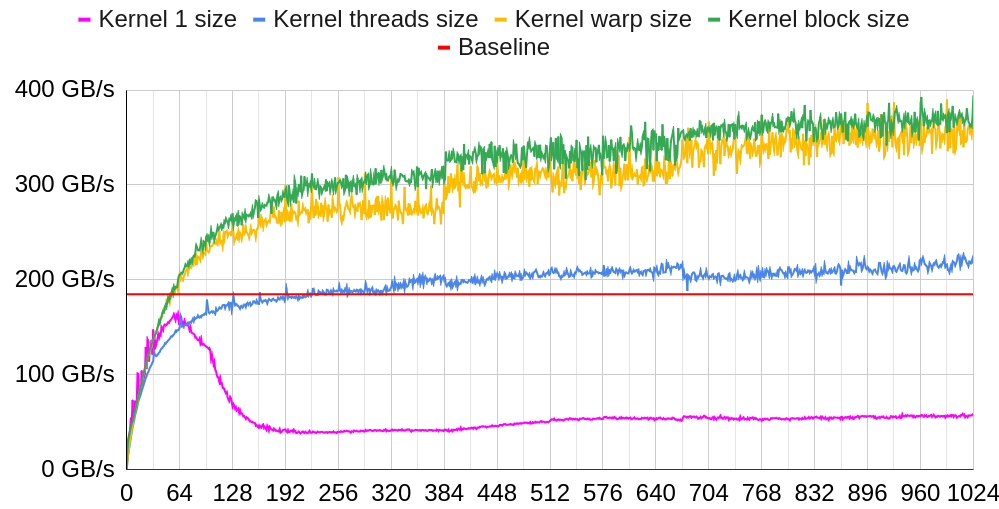
\includegraphics[width=1\linewidth]{data_images/Gb_for_size_block_2}
	\caption{Throughput over block size of the various kernels}
	\label{fig:gbforsizeblock2}
\end{figure}


\begin{figure}[h!]
	\centering
	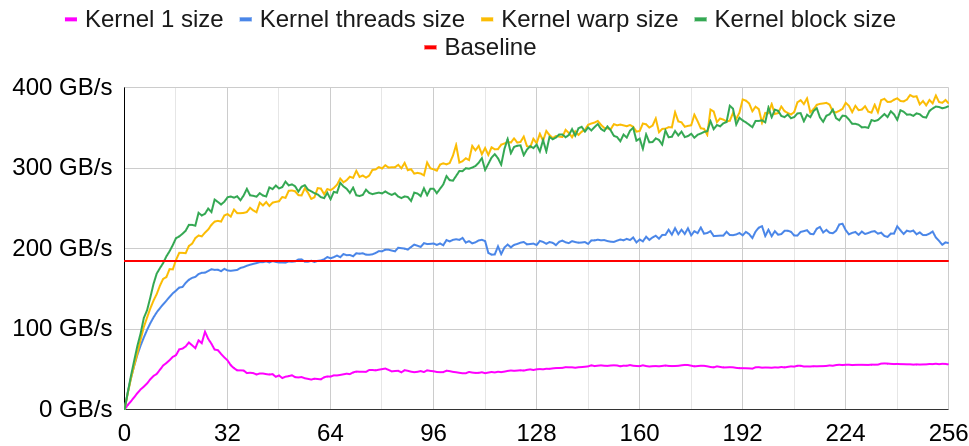
\includegraphics[width=1\linewidth]{data_images/Gb_for_size_grid_2}
	\caption{Throughput over blocks number of the various kernels}
	\label{fig:gbforsizegrid2}
\end{figure}

\FloatBarrier
Also as expected the two graph look very alike. That is because the A30 has only 4 SM with each a warp of size 32, so increasing to values above this value, has similar result if it is done via block size or number of blocks.

The kernels were then benchmarked with all the datasets, using the best parameter, those being 1024 threads for blocks and with 256 blocks.

\begin{figure}[h!]
	\centering
	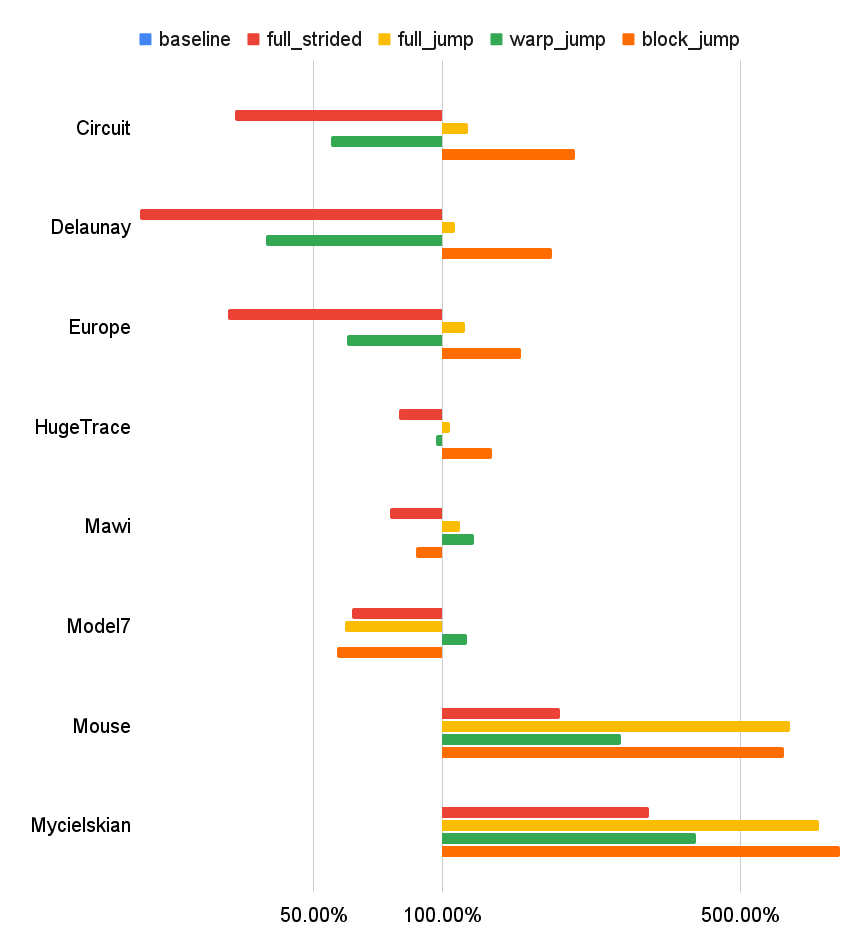
\includegraphics[width=0.9\linewidth]{data_images/perf_gpu}
	\caption{Performance of the kernels based on dataset}
	\label{fig:perf-gpu}
\end{figure}
% TODO Insert (9 e 10) general on all kernels
% https://docs.google.com/spreadsheets/d/1zCtsu4Ix58ZK-W56i8j56o1_yVpRHqyXO1a4qWqDquE/edit?gid=0#gid=0
% https://docs.google.com/spreadsheets/d/1M4LpwCNj--Tn50xUVJOkwcCPsH2g87JFIn6aph0HDnE/edit?gid=0#gid=0
\FloatBarrier


\todo{Comparison with CPU perf}

As it was expected, the worst performance come from the smallest dataset. The cause of this, is that GPU are optimized for throughput and so they have higher latency. So with smaller size datasets the latency become the limiting factor. It can also be noted that on small datasets the comparison between the various kernel become meaningless, as the time is almost all spent on the various overhead (eg. creating a kernel).


\begin{table}[h!]
	\centering
	\begin{adjustbox}{width=\columnwidth}
		\begin{tabular}{lcccc}
			\toprule
			\textbf{Kernel} & \textbf{Mawi} & \textbf{Delaunay} & \textbf{Circuit5c} & \textbf{Model7}\\
			\midrule
			Kernel 1 size & 15.1 GB/s & 46.7 GB/s & 56.1 GB/s & 4.08 GB/s\\
			Kernel threads size GB/s & 19.8 GB/s & 136 GB/s & 202 GB/s & 3.6 GB/s\\
			Kernel warp size & 20.5 GB/s & 198 GB/s & 361 GB/s & 3.74 GB/s\\
			Kernel blocks size & 21.1 GB/s & 172 GB/s & 341 GB/s & 2.8 GB/s\\
			\bottomrule
		\end{tabular}
	\end{adjustbox}
	\vspace{1em}

	\caption{Results in table format}
	\label{tab:gpu-results}
\end{table}

\FloatBarrier

Finally we can node how, ignoring Model7, the "Kernel warp size" has the most reliable performance as expected while sometimes the "Kernel block size" has better performance but is not very reliable, having a larger variance.


\section{Conclusions}
In conclusion COO present various problematic aspect when talking about parallelization, requiring atomic operation, in contrast to the CSR implementation. Because of this, the performance obtained are even worse than the theoretical worse case as it was theorized.



\begin{figure}[hbt!]
	\centering
	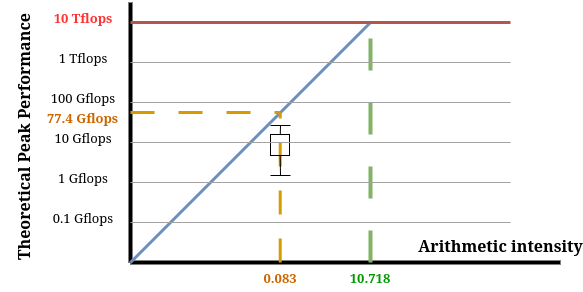
\includegraphics[width=1\linewidth]{data_images/roofline}
	\caption{Roofline model of a NVIDIA A30}
	\label{fig:roofline}
\end{figure}

This can be seen in Image \ref{fig:roofline} . To be exact the best result obtained is only $37\%$ of the theoretical worst case scenario.
\\

In conclusion, we can assert that COO is not suitable representation for sparse matrix when talking about efficient kernel implementation, especially in the case of a naive implementation. In such cases, it should be instead evaluated the use of CSR.
\end{document}

